\section{Séance 7}

\paragraph{1. } Lorsqu'on réalise un exposé oral il faut choisir soigneusement ses notations afin d'éviter les confusions sonores entre lettres (comme entre $m$ et $n$ par exemple). Dans un alphabet de $N$ lettres, on a identifié toutes les paires de lettres qu'il est possible de confondre et on aimerait sélectionner un ensemble de lettres pour nos notations de sorte qu'aucune confusion ne soit possible.
\begin{enumerate}
  \item[a.] Modélisez cette situation comme un problème de graphes. Comment trouver le plus grand nombre de lettres non-confondables possible?
  \item[b.] On a besoin de $r$ symboles pour notre présentation. A partir de combien de couples de lettres confondables risque-t-on de devoir utiliser des symboles pouvant prêter à confusion?
\end{enumerate}


\paragraph{2. } Dans un groupe de 9 personnes, une personne connait 2 autres personnes, ces 2 personnes connaissent chacune 4 personnes, 4 personnes connaissent chacune 5 personnes et les 2 dernières personnes connaissent chacune 6 personnes. Montrez qu'il existe 3 personnes qui se connaissent l'une l'autre.


\paragraph{3. } Une fête regroupe $n$ personnes, chacune ayant au moins un ami présent (l'amitié étant réciproque). Dans tout groupe d'au moins 3 personnes, il n'y a jamais exactement 2 paires d'amis. Prouvez que chaque personne est amie avec toutes les autres.

\begin{solution}
Si l'on représente les amis par des nœuds et leurs amitiés par les arêtes, les seuls sous-graphes à 3 nœuds possibles (pour éviter d'avoir exactement deux paires d'amis dans un sous-graphe) sont les suivants:

\begin{center}
\begin{tikzpicture}
\GraphInit[vstyle=Normal]
\SetGraphUnit{1}
\begin{scope}[rotate=90]
\Vertices{circle}{$a$,$b$,$c$}
\end{scope}
\Edges($a$,$b$,$c$,$a$)
\end{tikzpicture}
\hspace*{2cm}
\begin{tikzpicture}
\GraphInit[vstyle=Normal]
\SetGraphUnit{1}
\begin{scope}[rotate=90]
\Vertices{circle}{$a$,$b$,$c$}
\end{scope}
\Edges($a$,$b$)
\end{tikzpicture}
\hspace*{2cm}
\begin{tikzpicture}
\GraphInit[vstyle=Normal]
\SetGraphUnit{1}
\begin{scope}[rotate=90]
\Vertices{circle}{$a$,$b$,$c$}
\end{scope}
\end{tikzpicture}
\end{center}

Si l'on prend un graphe à 3 nœuds, tout le monde est ami, car chaque personne a au moins un ami présent.

\begin{center}
\begin{tikzpicture}
\GraphInit[vstyle=Normal]
\SetGraphUnit{1}
\begin{scope}[rotate=90]
\Vertices{circle}{$a$,$b$,$c$}
\end{scope}
\Edges($a$,$b$,$c$,$a$)
\end{tikzpicture}
\end{center}

Ajoutons un nœud $d$, il doit forcément être connecté à un des nœuds existant déjà (par exemple le nœud $a$) puisque chaque personne a un ami présent.

\begin{center}
\begin{tikzpicture}
\GraphInit[vstyle=Normal]
\SetGraphUnit{1}
\begin{scope}[rotate=90]
\Vertices{circle}{$a$,$b$,$c$,$d$}
\end{scope}
\Edges($a$,$b$,$c$,$a$)
\SetUpEdge[color=green]
\Edges($a$,$d$)
\end{tikzpicture}
\end{center}

Dans ce nouveau graphe, tout ensemble de trois nœuds contenant $a$ et $d$ possède 2 arêtes puisque le troisième nœud est connecté à $a$. Ceci contredit l'hypothèse selon laquelle dans tout graphe d'au moins 3 personnes, il n'y a jamais exactement 2 paires d'amis, ce qui signifie qu'il faut relier $d$ au troisième nœud. Le même raisonnement s'applique à tout ensemble de 3 nœuds du graphe contenant $a$ et $d$. Par conséquent, $d$ doit être relié à tous les nœuds du graphe.

\begin{center}
\begin{tikzpicture}
\GraphInit[vstyle=Normal]
\SetGraphUnit{1}
\begin{scope}[rotate=90]
\Vertices{circle}{$a$,$b$,$c$,$d$}
\end{scope}
\Edges($a$,$b$,$c$,$a$)
\SetUpEdge[color=green]
\Edges($a$,$d$)
\SetUpEdge[color=red]
\Edges($b$,$d$,$c$)
\end{tikzpicture}
\end{center}

Cette preuve s'applique pour chaque nouvel ajout de nœuds au graphe. On en conclut que dans un graphe de $n$ nœuds, chaque personne est amie avec toutes les autres.
\end{solution}

\paragraph{4. } Montrez que le graphe $G$ est biparti si et seulement si $\alpha(H) \geq \frac{1}{2} \nu(H)$ pour tout sous-graphe $H$ de $G$.
\begin{itemize}
  \item $\alpha(H)$ est le nombre de sommets dans un ensemble indépendant maximum de $H$;
  \item $\nu(H)$ est le nombre de sommets de $H$.
\end{itemize}


\paragraph{5. } Sans utiliser le Théorème de Turán, montrez que si le graphe $G = (V, E)$ est simple et que $|E| > \frac{|V|^2}{4}$, alors $G$ contient un triangle.
